\documentclass[12pt]{article}
%\usepackage[]{geometry}
\usepackage[top=1in,bottom=1in,left=1in,right=1in]{geometry}
\usepackage[utf8]{inputenc}
\usepackage{graphicx}
\usepackage{hyperref}

\title{IED Project\\
        Room mapping mini-bots}
\author{
    Ghosal, Radhika\\
    \texttt{radhika15160@iiitd.ac.in}
    \and
    Luthra, Jai\\
    \texttt{jai15043@iiitd.ac.in}
    \and
    Mittal, Parth\\
    \texttt{parth15069@iiitd.ac.in}
    \and
    Talwar, Divyanshu\\
    \texttt{divyanshu15028@iiitd.ac.in}
}

\begin{document}

\maketitle
\tableofcontents

\pagebreak

\section{Functional Block Diagram}
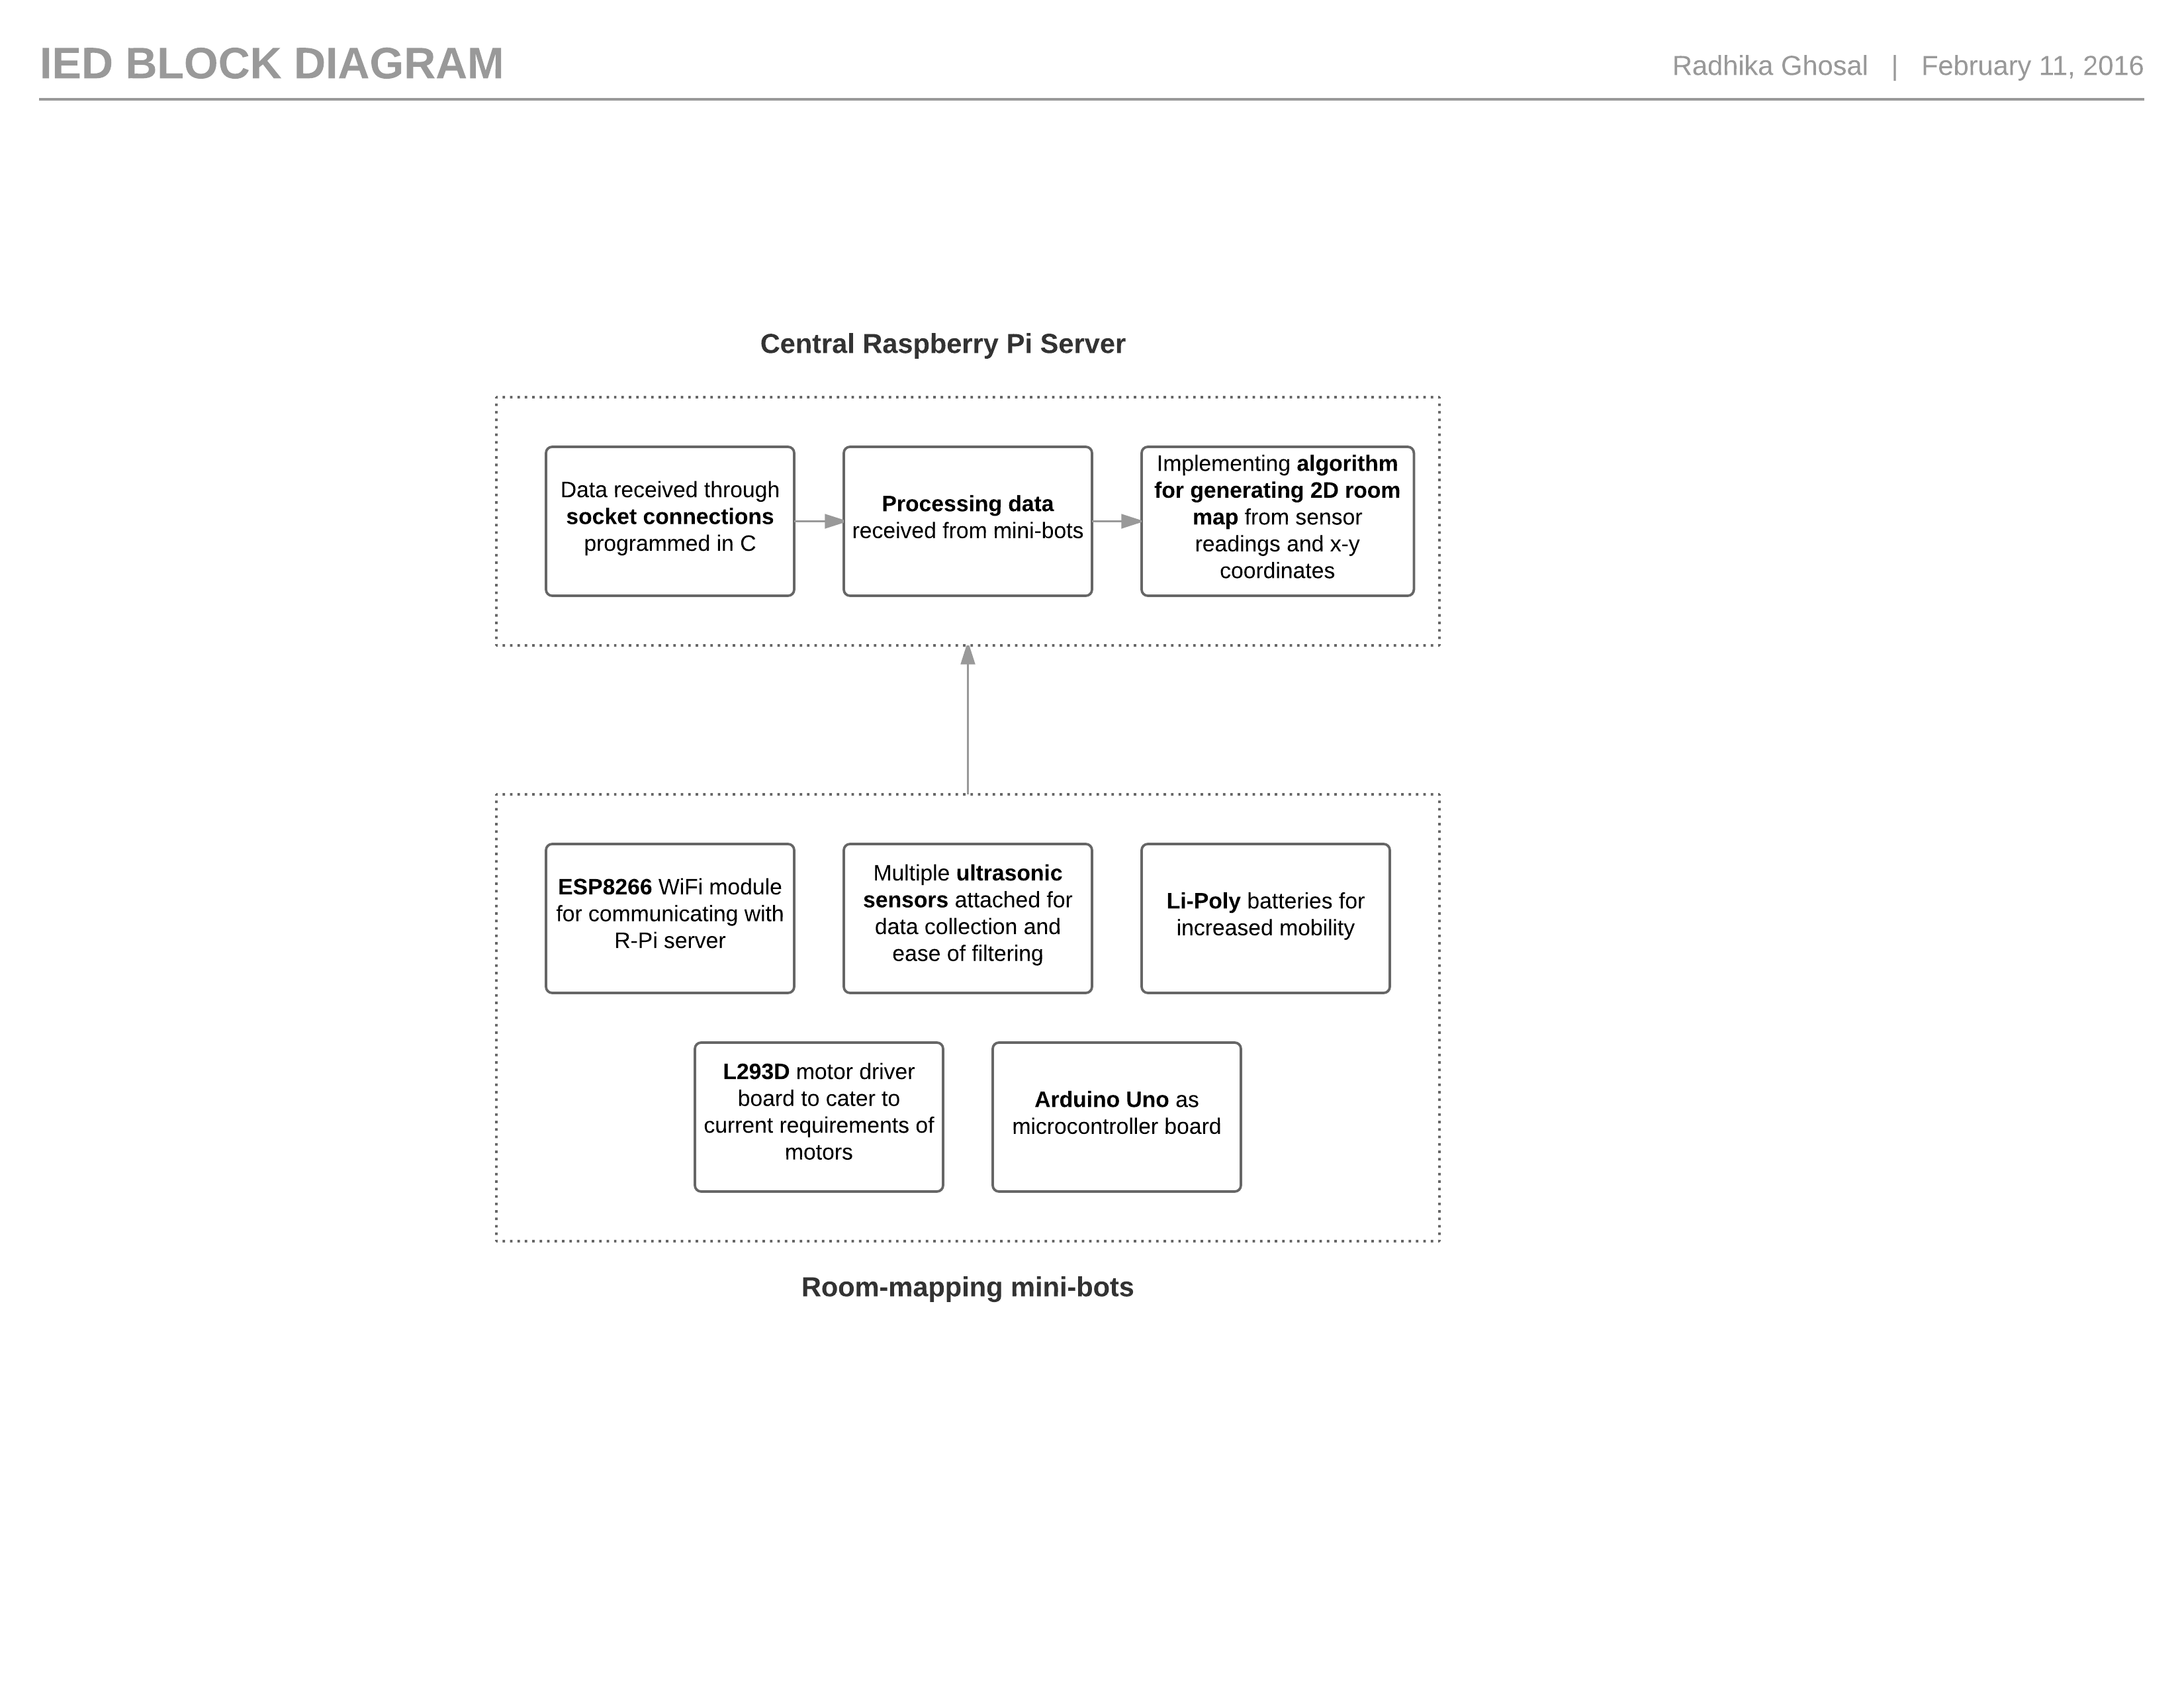
\includegraphics[width=\textwidth]{blockdiag.png}

\pagebreak

\section{Tentative Bill of Materials}

\begin{itemize}
    \item
		Raspberry Pi $\times 1$ (for the server)
	\item
		Li-Poly Battery Charger $\times 1$ \hfill \textit{Rs.999}
    \item
        \textbf{Per map-bot}
        \begin{itemize}
        \item
            Arduino Uno $\times 1$
        \item
			Ultrasound sensor [HC-SR04] $\times 4$ \hfill \textit{Rs. 680}
        \item
            Caster wheel $\times 1$ \hfill \textit{Rs. 40}
        \item
            DC Motors $\times 2$ \hfill \textit{Rs. 300}
        \item
            Wi-fi module [ESP8266] $\times 1$
        \item
            Wheel encoder kit $\times 2$ \hfill \textit{Rs. 600}
        \item
            L293D Motor Driver Board $\times 1$ \hfill \textit{Rs. 120}
        \item
            Chassis $\times 1$ \hfill \textit{Rs. 80}
        \item
            I2C Logic Level Converter $\times 1$
		\item
			Li-Poly Battery (7.4V, 1600MAh) $\times 1$ \hfill \textit{Rs.600}
		\item
			\textbf{Total \hfill \textit{Rs.2420}}
        \end{itemize}
\end{itemize}

\textbf{Sources:} \href{http://www.nex-robotics.com}{Nex-Robotics}, \href{https://www.robomart.com/}{Robomart}

\section{Initial Approach}

We will attempt to solve the Indoor Localization Problem, by developing a robust procedure to create maps of indoor environments from readings off multiple sonar devices, specifically, by using ultrasonic sensors.\\
\\
Our setup currently consists of a basic client-server system, where we will be using a Raspberry Pi as a server, and the map-bots as clients. 
We will be setting up a local IP address and a server on the R-Pi for the ESP8266 onboard the map-bots, to send and receive serial data and 
x-y coordinates from the robots. Main processing of information will happen on the Raspberry Pi, ensuring that we can write all the 
map-generation code in a high level language like C++.\\
\\
Our intial aim is to get two bots working, and then extend our method to multiple bots.


\section{Problematic sub-problems}
\subsection{Odometric error}
    
A large part of the localization problem is the errors that accumulate from most methods of odometry. This is discussed in great detail in \cite{tardos}, and they develop a robust algorithm which manages to reduce the mapping error to that of the sonar sensor. 

\subsection{Autonomous routing}

Developing an algorithm which minimizes turning (to minimize odometric error from skidding), and yet manages to map an environment fairly quickly appears to be non-trivial. 

\subsection{Extension to multiple bots}

Extending said hypothetical autonomous routing algorithm to multiple bots while minimizing redundancy also seems non-trivial.

\section{Timeline}

\subsection{February}

\begin{itemize}
    \item
        Two bots should be moving and collecting data.
        \begin{itemize}
        \item
            \underline{Week 1:} Should move according to a pre-programmed sketch.
        \item
            \underline{Week 2:} Should track its displacement from its original
            position using the wheel encoder, without errors from skidding and turning.
        \item
            \underline{Week 3:} Should read and transfer serial data from sensors and
            x-y coordinates to the R-Pi server.
        \item
            \underline{Week 4:} Should move autonomously through the room with a
            \textit{random-walk} motion and collision detection.
        \end{itemize}

    \item
        \underline{Week 3:} R-Pi server should be ready for data transfer.
    \item
        \underline{Week 4:} A minimal algorithm for map-generation should be ready, at least on paper.
\end{itemize}

\subsection{March}

\begin{itemize}
    \item
        \underline{Week 1:} Should definitely have enough sensor readings and x-y coordinates for
        an entire room to start testing and improving upon the map-generation
        algorithm.
        
    \item
        \underline{Week 4:} Should have a working autonomous routing algorithm, and have it tested thoroughly
        for different rooms.

\end{itemize}

\begin{thebibliography}{1}

\bibitem{tardos}
Juan D. Tardós, José Neira, Paul M. Newman, and John J. Leonard.
\textit{Robust Mapping and Localization in Indoor Environments Using Sonar Data}
\end{thebibliography}

\end{document}
